\chapter{Introduction}
\label{cha:intro}
The first contains a general introduction to the work. The goals are
defined and the modus operandi is explained.
\todo{bib referenties in orde brengen}
\section{Introduction}

Security is an important asset in Computer Science. Defending a network of a company is not an easy job. To prevent intruders it can make use of firewalls, routers, IDS systems, virus scans, and other defence mechanisms. Unfortunately technology is growing fast and attacks are getting more sophisticated and the causes of these attacks can be very different. \todo{iets tussen nog} Companies are often the victim of targeted attacks. In a security report of 2014, \todo{verwijzing naar report}, states that 80\% of the companies are the victims of targeted attacks. Many companies don't see themselves as a target, but sometimes they might be collateral, the target on the way to the real target. This means that everybody can be a target. 
Corporate networks should continuously defend themselves against outside invaders such as viruses and worms. By doing so the network administrator can keep the network as malware-free as possible. If there is  an intruder managed to penetrate the network then the network manager this intruder trying to get out as quickly as possible. This is not always easy. Especially when the intruders secretly sneak and then spread rapidly.
In this paper we will work further on the work made by Marten van Dijk, Ari Juels, Alina Oprea and Ronals L. Rivest \todo{verwijzing naar FlipIT} who wrote a report on the Game FlipIt. FlipIt is a the game of '' Stealthy Takeovers''. It models a game by means of two players, the attacker and the defender. Both can gain control over a single shared resource by flipping it. The most important property of the game is that the flipping happens stealthy. This means that the players have no clue about when the other player moves. The goal of the game is to maximise the time the player controls the resource minus the average cost of the flipping. 

\subsection{Motivation of the game}
%waarom FlipIt gebruiken en niet iets anders.
\subsection{Contributions and results}
\subsection{Conclusions}
The "I love you" virus is an example of a virus that spreads quickly. This virus propagates via mail systems. If someone opens an email with "I love you" virus in annex this virus spreads itself by sending a mail itself to everyone in your contact list. So the virus can multiply rapidly and eventually a business network shut down by the heavy traffic. In this example, there is a need human interaction to spread the virus to do. If no one opens the virus can not spread the mail.
Unfortunately, there are viruses that can spread without human interaction. These viruses are referred to as worms. A worm is also a computer program that replicates itself to spread to other computers so. Via a computer network, copies of the worm forwarded without an intermediary is used for. The worm will use vulnerabilities to infect other computers.
Most worms are designed to spread out and just try not to make any changes to the systems that they pass. These worms can still inflict damage by increased network traffic they generate. Worms that contain Harm damage a program to install a backdoor or a rootkit on the infected computers. Backdoors and rootkits ensure that future use can be made of the infected computers.
The Stuxnetworm is a very famous worm. Initially this worm spread via infected USB sticks and from then it could spread through the Internet to other computers. The purpose of the Stuxnetworm was broken to run the centrifuges in nuclear reactors. Many reactors have been infected. From the standpoint of the defender, it is very important to respond as quickly as possible so that the worm can not spread quickly.

\section{introduction number 2}

(We live in an era) In this era where digitalization becomes prominent in every aspect of our lives, where technology is growing fast and where business are always under attack, security becomes an issue of increasing complexity. Since 2009, the number of reported security attacks on companies has increased 66\%, year over year. \todo{security report van pwc}. These numbers only represent the attacks that are detected. In 2014 117,339 attacks where coming in daily. Many of those attacks have a different cause. Some of them can be benign, others can be harmful. Many companies are unaware of all the attacks. Some of them think that they are not a target, but they might be a target on the way to a real target. Recently there where some high profiled targeted attacks which have been revealed. (Belgacom). 
Targeted attacks are ...
The \textit{Kill Chain} is a concept by Lockheed Martin Corporation, explained in the whitepaper \todo{withepaper toevoegen}. It explains the different phases of a typical attack from the view of an attacker. It also outlines the typical attacker activities on the right. This model is very useful to define the different moments of the life cycle of an attack and when a company should act to defend itself. In this paper we would like to prevent the viruses of spreading into the network system of a company. This means that we have to act in phase Installation, Command and Control and Action on Objectives of the kill chain. 

 
  Security is an important asset in Computer Science. Defending a network of a company is not an easy job. Malicious people will try to  To prevent intruders it can make use of firewalls, routers, IDS systems, virus scans, and other defence mechanisms. Unfortunately technology is growing fast and attacks are getting more sophisticated and the causes of these attacks can be very different. \todo{iets tussen nog} Companies are often the victim of targeted attacks. In a security report of 2014, \todo{verwijzing naar report}, states that 80\% of the companies are the victims of targeted attacks. Many companies don't see themselves as a target, but sometimes they might be collateral, the target on the way to the real target. This means that everybody can be a target. 
Corporate networks should continuously defend themselves against outside invaders and targeted attacks. Researchers have already investigated the situations through the FlipIt game in which a system is continuously compromised by an attacker through targeted attacks. 
FlipIt is a the game of '' Stealthy Takeovers''. It models a game by means of two players, the attacker and the defender. Both can gain control over a single shared resource by flipping it. The most important property of the game is that the flipping happens stealthy. This means that the players have no clue about when the other player moves and has control over the shared resource. The goal of the game is to maximise the time the player controls the resource minus the average cost of the number of flipping.
In this paper we model a company network through multiple shared resources and a flip from the attacker that drops a virus that will spread itself autonomously. We show that ...

%\begin{minipage}{0.5\textwidth}
%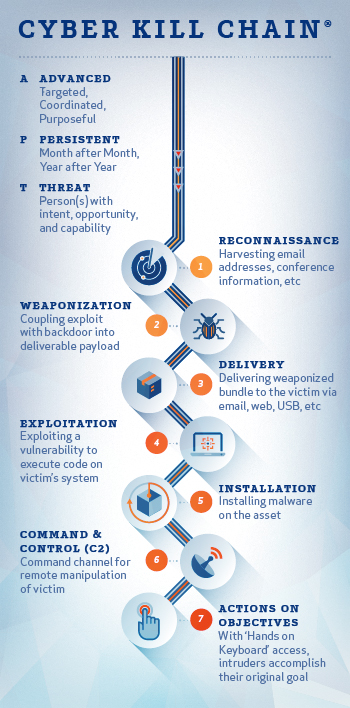
\includegraphics{Images/killchain.jpg}
%\end{minipage} \hfill
%\begin{minipage}{0.45\textwidth}
%\begin{itemize}
%\item *Rectangle
%\item *Color: blue
%\end{itemize}
%\end{minipage}

%http://www.pwc.com/gx/en/consulting-services/information-security-survey/index.jhtml
%%% Local Variables: 
%%% mode: latex
%%% TeX-master: "thesis"
%%% End: 
